\documentclass[sigconf]{acmart}
\settopmatter{printacmref=false}
\setcopyright{none}
\renewcommand\footnotetextcopyrightpermission[1]{}
\pagestyle{plain}

\usepackage{booktabs}
\usepackage{tikz}
\usetikzlibrary{positioning,fit,arrows.meta,calc}

% TODO camera-ready: real \country{} per author; BibTeX.

\begin{document}

\title{Team npatta01's Conversational Music Recommender for the RecSys Challenge 2026}

\author{Nidhin Pattaniyil}
\email{npatta01@gmail.com}
\affiliation{\institution{Independent Researcher}\country{USA}}

\author{Semih Yagli}
\email{semihyagli1@gmail.com}
\affiliation{\institution{Independent Researcher}\country{USA}}

\author{Tanwir Zaman}
\email{zaman.tanwir@gmail.com}
\affiliation{\institution{Independent Researcher}\country{USA}}

\begin{abstract}
We describe team npatta01's submission to the RecSys Challenge 2026 conversational music recommendation task: given a multi-turn dialog, retrieve 20 tracks from a 47,071-track catalog and generate a natural-language response. The pipeline extracts a typed conversation state with an LLM, gathers candidates from eleven retrieval branches over a single LanceDB collection, re-ranks the pooled candidates with a LightGBM LambdaMART model whose dominant feature is a fine-tuned conversational bi-encoder cosine, and generates a state-conditioned response. On the final Blind-B leaderboard the submission scored 0.3811 composite (nDCG@20 0.2537, LLM-judge 3.30), ranking 29th of 39 teams. We report the system in full, and then examine our own result: an in-sample development estimate (nDCG@20 0.38--0.46) created misplaced confidence while leakage-safe out-of-fold evidence (0.197--0.203) had already predicted the blind outcome; the benchmark's single-ground-truth labels carry a quantified \emph{anchoring bias} that teaches rankers to copy the just-played artist; and concrete failure cases from the submitted run show extracted constraints that the pipeline could not enforce. Code, models, and a zero-credential reproduction bundle: \url{https://github.com/npatta01/music-crs-2026}.
\end{abstract}

\maketitle

\section{Introduction}

The Music-CRS challenge~\cite{musiccrs,recsyschallenge2026} asks systems to act as a conversational music recommender. Each session is a multi-turn dialog between a listener and an assistant; at every assistant turn the system must (i)~retrieve a ranked list of 20 tracks from a shared 47,071-track catalog and (ii)~write a short natural-language response presenting its top recommendation. Training data comprises 15,199 sessions built on the TalkPlayData~2 collection~\cite{talkplay}, with per-track metadata (title, artist, album, up to 37 genre/mood tags, popularity, release date) and precomputed embeddings (text, audio, cover art, collaborative filtering). Evaluation is on two 80-session blind splits of final turns; Blind-B additionally removes the conversation-goal annotations present in training data. Submissions are scored with a composite metric:
\begin{displaymath}
0.50\cdot\text{nDCG@20} + 0.10\cdot\text{cat.\ div.} + 0.10\cdot\text{lex.\ div.} + 0.30\cdot\tfrac{\text{judge}-1}{4},
\end{displaymath}
where ``judge'' is a 1--5 LLM-as-a-judge rating of the generated response. A 1,000-session development split with public per-turn ground truth (one target track per turn) supports offline iteration.

Our system is a retrieve-then-rerank pipeline conditioned on an explicitly compiled conversation state. Per the challenge's participant-paper mandate we document the full pipeline (Section~\ref{sec:approach}) and results (Section~\ref{sec:experiments}); because we finished mid-pack, Section~\ref{sec:discussion} is an unusually frank retrospective. Contributions:
\begin{enumerate}
\item A complete, reproducible pipeline: LLM state extraction $\rightarrow$ eleven-branch retrieval over one LanceDB collection $\rightarrow$ LambdaMART re-ranking $\rightarrow$ state-conditioned response generation.
\item An evaluation-lineage lesson: our in-sample development replay (nDCG@20 0.38--0.46) drove selection confidence, while leakage-safe out-of-fold estimates (0.197--0.203) already anticipated the blind result (0.2537).
\item A fine-tuned conversational bi-encoder whose single cosine feature carries 59\% of the reranker's decision weight and replaces a label-noise-induced ``artist-copy'' shortcut.
\item A quantified analysis of ground-truth anchoring bias, with concrete failure cases from our submitted run and a cleaned, LLM-re-judged label set released alongside our code.
\end{enumerate}

Related work in brief: the design follows the retrieve-then-rerank pattern standard in large-catalog recommendation, with reciprocal-rank fusion~\cite{rrf} for multi-source pooling, LambdaMART~\cite{lightgbm,lambdamart} for learned ranking, and LLM-based dialog state tracking; the organizers' framework provided the evaluation harness.

\section{Approach}
\label{sec:approach}

\begin{figure*}[t]
  \centering
  \resizebox{\textwidth}{!}{%
  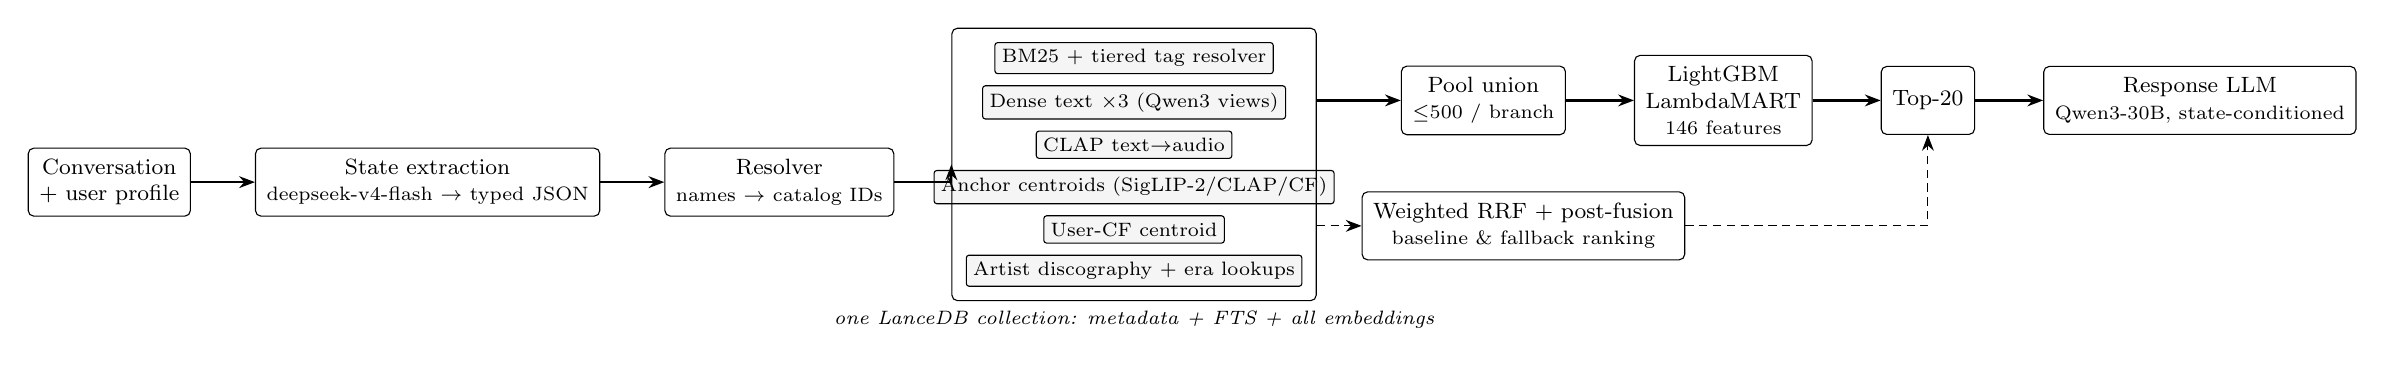
\begin{tikzpicture}[
    font=\footnotesize,
    box/.style={draw, rounded corners=2pt, align=center, inner sep=4pt, minimum height=0.34in},
    lane/.style={draw, rounded corners=1pt, align=left, inner sep=2.5pt, font=\scriptsize, fill=black!4},
    arr/.style={-{Stealth[length=2mm]}, thick},
    dasharr/.style={-{Stealth[length=2mm]}, densely dashed}
  ]
    \node[box] (conv) {Conversation\\+ user profile};
    \node[box, right=0.32in of conv] (state) {State extraction\\\scriptsize deepseek-v4-flash $\rightarrow$ typed JSON};
    \node[box, right=0.32in of state] (res) {Resolver\\\scriptsize names $\rightarrow$ catalog IDs};

    \node[lane, right=0.5in of res, yshift=0.62in] (l1) {BM25 + tiered tag resolver};
    \node[lane, below=0.055in of l1] (l2) {Dense text $\times$3 (Qwen3 views)};
    \node[lane, below=0.055in of l2] (l3) {CLAP text$\rightarrow$audio};
    \node[lane, below=0.055in of l3] (l4) {Anchor centroids (SigLIP-2/CLAP/CF)};
    \node[lane, below=0.055in of l4] (l5) {User-CF centroid};
    \node[lane, below=0.055in of l5] (l6) {Artist discography + era lookups};
    \node[draw, rounded corners=2pt, fit=(l1)(l6), inner sep=5pt, label={[font=\scriptsize\itshape]below:{one LanceDB collection: metadata + FTS + all embeddings}}] (branches) {};

    \node[box, right=0.42in of branches, yshift=0.32in] (union) {Pool union\\\scriptsize $\leq$500 / branch};
    \node[box, right=0.34in of union] (lgbm) {LightGBM\\LambdaMART\\\scriptsize 146 features};
    \node[box, right=0.34in of lgbm] (out) {Top-20};
    \node[box, right=0.34in of out] (resp) {Response LLM\\\scriptsize Qwen3-30B, state-conditioned};

    \node[box, below=0.28in of union, xshift=0.2in] (rrf) {Weighted RRF + post-fusion\\\scriptsize baseline \& fallback ranking};

    \draw[arr] (conv) -- (state);
    \draw[arr] (state) -- (res);
    \draw[arr] (res) -- (branches.west|-res) -- (branches.west);
    \draw[arr] (branches.east|-union) -- (union);
    \draw[arr] (union) -- (lgbm);
    \draw[arr] (lgbm) -- (out);
    \draw[arr] (out) -- (resp);
    \draw[dasharr] (branches.east|-rrf) -- (rrf);
    \draw[dasharr] (rrf.east) -| (out.south);
  \end{tikzpicture}%
  }
  \caption{System overview. The conversation is compiled into a typed state; eleven retrieval branches query one LanceDB collection; the LambdaMART reranker scores the branch-pool union and emits the top-20; a response LLM presents the top track. Weighted RRF over the same branches provides the baseline and fallback ranking (dashed).}
  \label{fig:pipeline}
\end{figure*}

\subsection{Understanding the conversation: state extraction}
\label{sec:state}

At each turn we prompt \texttt{deepseek-v4-flash} (via OpenRouter, JSON-schema constrained) to emit a typed conversation state, projected onto an 11-field contract: current request, intent mode (open-explore / refinement / pivot / playlist-build), per-track feedback with roles, mentioned entities, hard filters (release-date), explicit rejections (artist / track / tag), routing flags, lyrical theme, and a soft release-year range. A fuzzy resolver grounds surface names to catalog IDs so downstream stages operate on identifiers. Cheaper extraction models under-filled optional fields (rejections, attribute facets) in our checks, so all final runs use \texttt{deepseek-v4-flash}. Extraction runs once per turn and is cached.

\begin{figure}[t]
  \centering
  \fbox{\begin{minipage}{0.94\linewidth}\scriptsize
  \textbf{User (turn 3):} ``\ldots subdued, female singer, a sense of place in the lyrics, stark almost a cappella delivery\ldots not it either.''\\[2pt]
  \textbf{Extracted state (abridged):}\\
  \texttt{request\_type: hidden\_target}\\
  \texttt{anchor artist: Neko Case (must\_use)}\\
  \texttt{rejected tracks: "Calling Cards", "Man"}\\
  \texttt{facets: mood=subdued; lyrical\_theme=sense of place;}\\
  \texttt{\phantom{facets: }sonic=stark almost a cappella}\\[2pt]
  \textbf{Top-1:} Neko Case --- ``Bracing For Sunday''\\[2pt]
  \textbf{Submitted response:} ``You're looking for something subdued with a strong sense of place and a stark, almost a cappella delivery---and \emph{Bracing For Sunday} fits that mood perfectly. Neko Case's haunting, intimate vocals carry the weight of a quiet, specific moment\ldots''
  \end{minipage}}
  \caption{A real Blind-B turn (session \texttt{024a2738\ldots}): extracted state and submitted output for a hidden-target request.}
  \label{fig:example}
\end{figure}

\subsection{Gathering candidates: one collection, eleven branches}
\label{sec:retrieval}

All per-track information lives in a \textbf{single LanceDB collection}: metadata fields, a Tantivy full-text index, and every embedding column --- three Qwen3-Embedding text views (metadata, attributes, lyrics; 1024-d), LAION-CLAP audio (512-d)~\cite{clap}, SigLIP-2 cover art (768-d)~\cite{siglip2}, BPR collaborative-filtering vectors (128-d)~\cite{bpr}, and our bi-encoder document vectors (2560-d, Section~\ref{sec:biencoder}). Every retrieval branch is a differently-shaped query against the same table --- in principle the whole retrieval step could be one composed query clause (Section~\ref{sec:fellshort}).

Eleven branches produce candidate pools per turn (Figure~\ref{fig:pipeline}): (1)~BM25~\cite{bm25} over title / artist / album / tags with field boosts, where free-text mood and genre phrases pass through a \textbf{tiered tag resolver} --- exact, alias, and substring matching against the catalog tag vocabulary with an embedding nearest-neighbor fallback (cosine $\geq 0.6$, top-3); (2--4)~dense ANN over the three Qwen3 text views; (5)~CLAP text-to-audio; (6--8)~centroids over liked anchor tracks in SigLIP-2, CLAP, and CF-BPR space, gated by intent mode (a pivot suppresses anchoring); (9)~the user's own CF vector; (10--11)~lookups from resolved-artist discographies and era popularity. Weighted reciprocal-rank fusion~\cite{rrf} ($k{=}60$, top-1000) plus post-fusion multiplicative adjustments (rejected artists/tracks dropped, played tracks dropped, exact-membership tag promotes/demotes, year-range decay) yields an explicit ranking that serves as \textbf{baseline and fallback}.

\subsection{Ranking with a learned model}
\label{sec:reranker}

The submitted system replaces the fused order entirely: a LightGBM LambdaMART~\cite{lightgbm,lambdamart} model scores the \textbf{union of the branch pools} (each truncated to its top 500) and emits the final top-20. It sees 146 features per (turn, track) pair: per-branch rank/score/margin/hit features, pool-normalized z-scores and percentiles, content and behavioral cosines, session/artist-affinity counters, tag and lexical overlap, popularity, extracted-state categoricals, and a constraint sidecar. Table~\ref{tab:families} groups them by family with each family's share of total split gain in the deployed model; one feature --- the bi-encoder cosine \texttt{b1\_cos} --- carries 59.0\% of all gain. The RRF rank itself is \emph{excluded}: the ranker sees raw branch evidence, not the fused opinion. After scoring, config-gated guards run (exact-track pins; a final-artist guard in the Blind-B configuration).

\begin{table}[t]
\caption{Reranker feature families (share of total gain, deployed model).}
\label{tab:families}
\small
\begin{tabular}{lrrl}
\toprule
Family & \# & Gain & Examples \\
\midrule
Bi-encoder cosine & 1 & 59.0\% & \texttt{b1\_cos} \\
Per-branch rank/score & 66 & 11.5\% & BM25 rank, dense margins \\
Session/artist affinity & 18 & 10.7\% & same-artist, played count \\
Other similarity cosines & 17 & 8.9\% & CLAP/SigLIP centroids \\
Popularity & 7 & 5.0\% & pop.\ percentile \\
State/intent & 14 & 2.2\% & request type, intent mode \\
Tag/lexical overlap & 10 & 2.0\% & IDF tag overlap \\
Constraints/rejections & 13 & 0.7\% & rejected-artist flag \\
\bottomrule
\end{tabular}
\end{table}

Training uses the per-turn ground-truth track as a binary label (LambdaRank objective optimizing nDCG@20; learning rate 0.025; 127 leaves; truncation 200; 5-fold user-grouped cross-validation; ${\sim}20.6$M rows). Because the ground truth is noisy (Section~\ref{sec:groundtruth}), labels are down-weighted when the \emph{next} turn contradicts them: $\times 0.3$ if goal progress says the recommendation did not move toward the goal, $\times 0.3$ if the user rejects the ground-truth track, $\times 0.6$ if they reject its artist. The deployed bundle is \emph{goal-free}: trained without the conversation-goal fields Blind-B removes. Cost shaped the training set: state extraction and per-turn retrieval tracing run through a paid LLM API, so the model trains on a 30,000-turn subset (${\sim}25\%$ of the ${\sim}121.6$k-turn split); the data-scaling curve had not flattened at that size.

\subsection{The conversational bi-encoder behind \texttt{b1\_cos}}
\label{sec:biencoder}

\begin{figure}[t]
  \centering
  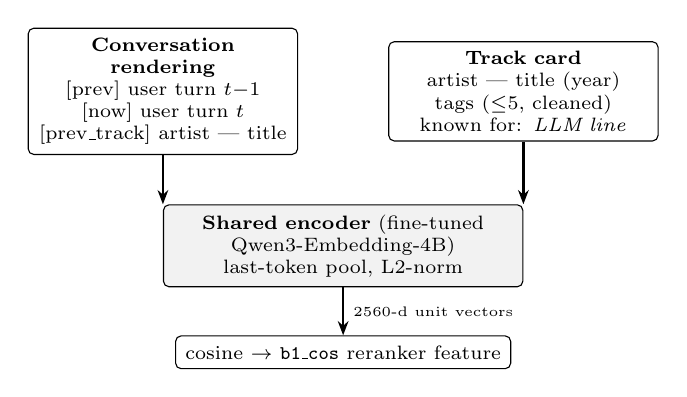
\begin{tikzpicture}[
    font=\scriptsize,
    box/.style={draw, rounded corners=2pt, align=center, inner sep=3.5pt},
    arr/.style={-{Stealth[length=1.8mm]}, thick}
  ]
    \node[box, text width=1.25in] (q) {\textbf{Conversation rendering}\\{[prev]} user turn $t{-}1$\\{[now]} user turn $t$\\{[prev\_track]} artist --- title};
    \node[box, text width=1.25in, right=0.45in of q] (d) {\textbf{Track card}\\artist --- title (year)\\tags ($\leq$5, cleaned)\\known for: \emph{LLM line}};
    \node[box, below=0.28in of $(q.south)!0.5!(d.south)$, text width=1.7in, fill=black!5] (enc) {\textbf{Shared encoder} (fine-tuned Qwen3-Embedding-4B)\\last-token pool, L2-norm};
    \node[box, below=0.24in of enc] (cos) {cosine $\rightarrow$ \texttt{b1\_cos} reranker feature};
    \draw[arr] (q.south) -- (enc.north-|q.south);
    \draw[arr] (d.south) -- (enc.north-|d.south);
    \draw[arr] (enc) -- node[right, font=\tiny]{2560-d unit vectors} (cos);
  \end{tikzpicture}
  \caption{The b1 bi-encoder: one shared fine-tuned encoder embeds the conversation and the track card; their cosine is the reranker's dominant feature.}
  \label{fig:biencoder}
\end{figure}

The reranker's dominant feature comes from a two-tower bi-encoder fine-tuned from Qwen3-Embedding-4B~\cite{qwen3embedding} (Figure~\ref{fig:biencoder}). The query tower renders the conversation compactly behind a retrieval instruction prefix,
\begin{center}\small\texttt{[prev] $\langle$user turn $t{-}1$$\rangle$ [now] $\langle$user turn $t$$\rangle$ [prev\_track] $\langle$artist --- title$\rangle$},
\end{center}
and the document tower renders a track card,
\begin{center}\small\texttt{Music track: artist --- title (year) | tags: $\leq$5 | known for: $\langle$LLM line$\rangle$},
\end{center}
whose one-line LLM-written ``known for'' artist description imports static world knowledge from larger models into the embedding space. One shared encoder $E_\theta$ serves both towers; with $v_x = E_\theta(x)/\lVert E_\theta(x)\rVert_2$ (last-token pooling, 2560-d), the feature is the cosine $\texttt{b1\_cos}(q,d) = v_q^{\top} v_d$. Training minimizes the in-batch contrastive (MNRL) loss over batches of positive pairs $(q_i, d_i^{+})$ with four mined hard negatives per positive,
\begin{displaymath}
\mathcal{L} = -\tfrac{1}{B}\textstyle\sum_i \log \frac{\exp(v_{q_i}^{\top} v_{d_i^{+}}/\tau)}{\sum_{d \in \mathcal{D}_i} \exp(v_{q_i}^{\top} v_{d}/\tau)}, \qquad \tau = \tfrac{1}{20},
\end{displaymath}
where $\mathcal{D}_i$ contains the in-batch documents plus the hard negatives. Positives are conservative: the 53,885 (turn, track) pairs whose next-turn goal-progress annotation says the recommendation \emph{moved the session forward}. Document vectors for all 47,071 tracks are precomputed into the collection; the conversation vector is encoded live with caching.

We deploy the bi-encoder \emph{scout-only}: as a retrieval branch it added little coverage, but as a feature its cosine became the top signal (Table~\ref{tab:families}) --- and a \emph{generalizing replacement} for a shortcut learned from biased labels (Section~\ref{sec:groundtruth}): in leakage-safe out-of-fold ablations, removing the artist-consensus shortcut features reduces nDCG@20 by 0.0070, while adding \texttt{b1\_cos} more than recovers the loss ($+0.0091$) with the shortcut absent.

\subsection{Writing the response}
\label{sec:response}

The response generator is \texttt{Qwen3-30B-A3B-Instruct-2507}~\cite{qwen3} at temperature 0: a single pass over the top-1 track rendered as a delimited XML block ($\leq$10 tags; the delimiting stops the model from echoing raw metadata) plus the \emph{latest} extracted state. The deployed template's full style instruction is:
\begin{quote}\small\itshape
``Write 1--2 concise sentences about only the selected track. Prioritize the latest user request and extracted state over older conversation history. If the track is reasonably aligned, explain the fit with one specific supported reason. If it clearly conflicts with an explicit avoid/new-artist constraint, do not oversell it or blame the system; briefly frame the limitation and the closest supported reason.''
\end{quote}
Template choice matters: over a frozen Blind-A retrieval output, a sweep of eight templates moved the judge score from 3.95 to 4.70 without touching the recommendations. There is no multi-draft sampling, selection, fact-checking, or repair pass. On the development split we score retrieval only; both blind submissions use live generation.

Code, configs, trained models, cached extraction states, and a frozen-LLM-cache reproduction bundle that replays our submissions without API credentials are public.\footnote{\url{https://github.com/npatta01/music-crs-2026}; models and data: \url{https://huggingface.co/datasets/Npatta01/music-crs-repro-2026}.}

\section{Results}
\label{sec:experiments}

The development split (1,000 sessions $\times$ 8 turns) has one ground-truth track per turn, so Recall@k equals Hit@k. Table~\ref{tab:devset} reports development-split numbers \emph{with their evaluation lineage made explicit}; Table~\ref{tab:official} reports the official leaderboard results.

\begin{table}[t]
\caption{Development split, with evaluation lineage. The in-sample row replays turns the deployed (full-data) model saw during training; the out-of-fold rows are leakage-safe cross-validation estimates.}
\label{tab:devset}
\small
\begin{tabular}{lrr}
\toprule
System (lineage) & nDCG@20 & Hit@20 \\
\midrule
Weighted RRF fusion (no training) & 0.1492 & 0.3183 \\
LambdaMART, out-of-fold CV & 0.1970 & --- \\
\quad + \texttt{b1\_cos} (deployed feature set) & 0.2032 & --- \\
LambdaMART, \emph{in-sample replay} & 0.3844 & 0.5610 \\
\bottomrule
\end{tabular}
\par\smallskip
\parbox{\columnwidth}{\raggedright\footnotesize An earlier in-sample capture of the predecessor reranker model read 0.4562. Official Blind-B nDCG@20: 0.2537 --- between the out-of-fold estimates and far below the in-sample replay.}
\end{table}

\begin{table}[t]
\caption{Official CodaBench results; the composite formula is defined in Section~1.}
\label{tab:official}
\small
\begin{tabular}{lrrrrrr}
\toprule
Split & nDCG & Cat. & Lex. & Judge & Comp. & Rank \\
\midrule
Blind-A (dev) & 0.4380 & 0.0313 & 0.7670 & 4.20 & 0.5389 & --- \\
\textbf{Blind-B (final)} & 0.2537 & 0.0315 & 0.7862 & 3.30 & \textbf{0.3811} & \textbf{29/39} \\
\bottomrule
\end{tabular}
\end{table}

Read honestly, Table~\ref{tab:devset} says two things. Learned re-ranking over the pooled candidates does beat static fusion --- but by the leakage-safe estimate ($0.149 \rightarrow 0.197$--$0.203$), not by the in-sample replay ($\rightarrow 0.384$) that we watched during development. And the blind result (0.2537) is consistent with the out-of-fold evidence that was available before submission. Feature attribution is strikingly concentrated (Table~\ref{tab:families}): one learned similarity carries 59\% of gain, and classic signals (artist affinity, popularity) outweigh most hand-engineered lexical features.

\section{Retrospective: Where It Went Wrong}
\label{sec:discussion}

\subsection{Our development estimate was in-sample}
\label{sec:insample}

The deployed reranker was fit on all of its feature data (the CV folds informed early stopping, then a full-data model shipped), and our headline development numbers came from \emph{replaying splits the model had seen}. The resulting 0.38--0.46 development estimates drove selection confidence; the leakage-safe out-of-fold numbers (0.197--0.203), which we had, predicted the blind outcome (0.2537) far better. We flag this as a measurement-and-confidence failure rather than a proven cause of the final ranking --- but it shaped every decision late in the competition, including which ideas looked ``already good enough'' to skip. The lesson is old but evidently worth restating: \emph{report and act on the out-of-fold number, even when the in-sample number is the one on the dashboard}.

\subsection{The ground truth contradicts itself}
\label{sec:groundtruth}

The benchmark's per-turn ground truth is a \emph{sibling pick} from the listener's real session --- the track actually played next --- not an editorial judgment of the request. In a manual sample only 62\% of ground-truth tracks were a clear fit to the request, 26\% a loose fit, and 11\% no fit. The dominant failure shape is \textbf{anchoring} (Figure~\ref{fig:contradiction}).

\begin{figure}[t]
  \centering
  \fbox{\begin{minipage}{0.94\linewidth}\scriptsize
  \textbf{User:} ``\ldots something with a similar chill, electronic vibe, but \textbf{from a different artist}?'' \hfill (just played: \emph{Bonobo})\\
  \textbf{Ground truth:} Bonobo --- ``Jets'' \hfill \emph{annotation: MOVES toward goal}\\[3pt]
  \textbf{User (next turn):} ``\,`Jets' is cool, but I was actually hoping for something \textbf{from a different artist this time}\ldots''\\
  \textbf{Ground truth:} Bonobo --- ``Pieces'' \hfill \emph{annotation: MOVES toward goal}
  \end{minipage}}
  \caption{Anchoring bias in the training labels (real session): two consecutive explicit different-artist requests, yet the ground truth stays on Bonobo and the synthetic reaction claims the listener liked it.}
  \label{fig:contradiction}
\end{figure}

To measure it we re-judged all 106,393 training turns (and 7,000 development turns) with an LLM pipeline: two inexpensive judges score each (request, ground-truth) pair on two axes --- did the user ask for a different artist, and does the track fit the request --- and a stronger arbiter re-judges conflicts \emph{blind to the synthetic reaction annotation}. Results: 57.4\% of turns judged negative; 18,222 are anchoring negatives; 5,880 of those carry a synthetic ``listener liked it'' annotation --- poisoned positives for any goal-progress-based training scheme, including our bi-encoder's. A second pattern --- the user rejects the ground-truth track on the next turn --- motivated our $\times 0.3$ label down-weighting. Anchored labels teach a specific wrong lesson: \emph{copy the last artist}. Our ablations show the ranker exploiting exactly this, and the bi-encoder cosine replacing the shortcut (Section~\ref{sec:biencoder}). Since every team is scored against the same labels, the bias depresses and partially reshuffles all measured scores. We release the cleaned relabeling with our code; the submitted models were \emph{not} trained on it.

\subsection{Failure cases from the submitted run}
\label{sec:failures}

A label-free LLM-judge audit of our 80 submitted Blind-B turns rated 68\% weak-or-bad fits; for 31 of 79 judged turns a better candidate was \emph{already in the retrieved pool} but ordered below the top-20 (versus 8 turns lost to over-aggressive filtering, 3 to state extraction, 1 to resolution) --- with the caveat that hidden-label frequencies are unknown. Concrete cases from the submitted predictions:

\begin{itemize}
\item \textbf{Anchoring at serving time.} ``Another alt-country song\ldots but \textbf{from a different artist than Ryan Adams}'' $\rightarrow$ our top-1 was \emph{Ryan Adams \& The Cardinals}, plus five more of their tracks in the top-20. The rejection resolved to the solo ``Ryan Adams'' catalog ID; the band-variant ID passed the hard-drop. The system reproduced exactly the bias of Section~\ref{sec:groundtruth}.
\item \textbf{Rejected artist in the list.} ``Symphonic black metal with strong \textbf{female operatic vocals}, \textbf{not Cradle of Filth}'' $\rightarrow$ four Cradle Of Filth tracks in the top-20 (a duplicate artist-ID variant escaped the drop), and the top-1 was a male-fronted power-metal track --- there is no vocal-attribute field to enforce.
\item \textbf{Impossible exact request.} ``Play `Watercolors' by Pat Metheny'' --- the track does not exist in the 47k catalog. We returned Pat Metheny's ``Alfie'' without acknowledging the gap; an honest ``that track is unavailable'' response would likely have scored better with the judge.
\item \textbf{Unactionable constraint.} ``Any aggressive metal track that \textbf{exactly matches 126.70 bpm and G minor}, with tempo and key stated'' --- the catalog has no BPM or key fields; the constraint could neither filter nor be verified, and the response could not state what the ask demanded.
\end{itemize}

\subsection{Where the pipeline lost information}
\label{sec:fellshort}

\paragraph{Rich extraction, uneven execution.} The state captured most of what users said, but each branch consumed only a slice of it and late fusion discarded the cross-field structure --- despite one collection making a single composed query (filters + text + vectors) possible. Tag handling illustrates it: the BM25 clause resolves free-text moods to canonical tags via the tiered resolver, yet post-fusion tag promotes/demotes and the reranker's overlap features use exact string membership, and only one soft feature (\texttt{tag\_emb\_cos}) sees semantic tag similarity.

\paragraph{Entity identity is fragmented.} Rejections were enforced by exact catalog ID, but artist identity in the catalog is not one ID per act (band variants, duplicates). Both leak cases above stem from this: a name-level or fuzzy-identity veto would have caught what the ID-exact drop missed.

\paragraph{No co-occurrence or transition evidence.} Behavioral signal entered only through CF-BPR centroids and lookups; the pipeline had no direct track-to-track co-occurrence or sequential-transition lane, and no LightGBM column can recreate a signal that never entered the pipeline.

\paragraph{Static knowledge, single-pass response.} LLM world knowledge entered only offline (the ``known for'' lines); nothing in the serving path reasons over candidates, which hidden-target requests (Figure~\ref{fig:example}) demand. The response was one temperature-0 draft with no selection, checking, or repair --- and at 30\% of the composite, our 3.30 judge score left the largest single block of points on the table.

\section{Conclusion}

We documented a state-compiled retrieve-then-rerank conversational music recommender in full, and audited our own mid-pack result honestly: an in-sample development estimate inflated confidence that leakage-safe evidence had already contradicted; the benchmark's single-label ground truth carries a quantified anchoring bias that our own submission reproduced at serving time; and several extracted constraints had no catalog fields or identity resolution to act on. We release the pipeline, models, a zero-credential replay bundle, and a cleaned relabeling of the training turns for future iterations.

\begin{thebibliography}{14}
\bibitem{musiccrs} NLP4MusA organizers. 2026. Music-CRS Challenge 2026. \url{https://nlp4musa.github.io/music-crs-challenge/}
\bibitem{recsyschallenge2026} RecSys Challenge 2026. \url{https://www.recsyschallenge.com/2026/}
\bibitem{talkplay} TalkPlay / TalkPlayData 2: multimodal conversational music recommendation dataset. \url{https://huggingface.co/collections/talkpl-ai/talkplay-data-challenge}
\bibitem{rrf} Gordon V. Cormack, Charles L. A. Clarke, and Stefan B\"uttcher. 2009. Reciprocal rank fusion outperforms Condorcet and individual rank learning methods. In \emph{SIGIR}.
\bibitem{lightgbm} Guolin Ke et al. 2017. LightGBM: a highly efficient gradient boosting decision tree. In \emph{NeurIPS}.
\bibitem{lambdamart} Christopher J. C. Burges. 2010. From RankNet to LambdaRank to LambdaMART: an overview. MSR-TR-2010-82.
\bibitem{qwen3embedding} Qwen Team. 2025. Qwen3 Embedding: advancing text embedding and reranking. arXiv:2506.05176.
\bibitem{clap} Yusong Wu et al. 2023. Large-scale contrastive language-audio pretraining. In \emph{ICASSP}.
\bibitem{siglip2} Michael Tschannen et al. 2025. SigLIP 2: multilingual vision-language encoders. arXiv:2502.14786.
\bibitem{bpr} Steffen Rendle et al. 2009. BPR: Bayesian personalized ranking from implicit feedback. In \emph{UAI}.
\bibitem{bm25} Stephen Robertson and Hugo Zaragoza. 2009. The probabilistic relevance framework: BM25 and beyond. \emph{Foundations and Trends in IR}.
\bibitem{qwen3} Qwen Team. 2025. Qwen3 technical report. arXiv:2505.09388.
\bibitem{deepseek} DeepSeek. 2026. DeepSeek-V4-Flash model card (OpenRouter).
\bibitem{lancedb} LanceDB: serverless vector database. \url{https://lancedb.com}
\end{thebibliography}

\end{document}
